\documentclass[11pt]{article}
\usepackage[sc]{mathpazo} %Like Palatino with extensive math support
\usepackage{fullpage}
\usepackage[authoryear,sectionbib,sort]{natbib}
\linespread{1.7}
\usepackage[utf8]{inputenc}
\usepackage{lineno}
\usepackage{amsmath, amsthm}
\usepackage{graphicx,hyperref}
\usepackage{microtype, parskip}
\usepackage[font=small]{caption}
\usepackage{float}
\usepackage{subcaption, multirow, morefloats}
\usepackage{wrapfig}
\usepackage{afterpage}
\usepackage{rotating}
\usepackage{lineno}

%%%%%%%%%%%%%%%%%%%%%
% LaTeX packages
%%%%%%%%%%%%%%%%%%%%%
% Please be sparing in your use of additional LaTeX packages, and
% upload any required style files to Editorial Manager with the file
% type "LaTeX ancillary files (.sty, .bst)."

%%%%%%%%%%%%%%%%%%%%%
% Line numbering
%%%%%%%%%%%%%%%%%%%%%
\usepackage{lineno}
% Please use line numbering with your initial submission and
% subsequent revisions. After acceptance, please comment out 
% the commands \usepackage{lineno}, \linenumbers{} 
% and \modulolinenumbers[3] below.

\title{Ensemble approaches for estimating congruence between species delimitation and morphological variation: comparing taxonomic hypotheses for the Pacific Pond Turtle (\textit{Emys marmorata})}

%%%%%%%%%%%%%%%%%%%%%
% Authorship
%%%%%%%%%%%%%%%%%%%%%
% Please remove authorship information while your paper is under review,
% unless you wish to waive your anonymity under double-blind review. 
% Remember to uncomment the information after acceptance.

\author{Peter D Smits$^{1,\ast,\dag}$ \\ 
Kenneth D Angielczyk$^{2}$ \\ 
Bryan L Stuart$^{3}$ \\
James F Parham$^{4}$}

\date{}

\begin{document}
% The journal does not have numbered sections in the main portion of
% articles. Please refrain from using section references such as
% section~\ref{section:CountingOwlEggs}, and refer to sections by name
% (e.g. section ``Counting Owl Eggs'').

% Please note that we prefer (\citealt{Xiao2015}) to \citep{Xiao2015},
% since \citep{} inserts a comma after "et al."

\maketitle

\noindent{}1. Department of Integrative Biology, University of California -- Berkeley, Berkeley, CA, USA;

\noindent{}2. Integrative Research Center, Field Museum of Natural History, Chicago, IL, USA;

\noindent{}3. Section of Research and Collections, North Carolina Museum of Natural Sciences, Raleigh, NC, USA;

\noindent{}4. John D. Cooper Archaeological and Paleontological Center, Department of Geological Sciences, California State University Fullerton, Fullerton, CA, USA.


\noindent{}$\ast$ Corresponding author; e-mail: psmits@berkeley.edu

\noindent{}$\dag$ ORCIDs: Smits, 0000-0003-4074-1447.

\bigskip

\textit{Manuscript elements}: Figure~1, figure~2, figure~3, figure~4, figure~5, figure~6, figure~7, figure~8, figure~9, table~1, table~2, table~3. Figures 1, 3, 4, 6, 8 are in color.

\bigskip

\textit{Keywords}: Geometric morphometrics, machine learning, conservation, Testudinae.

\bigskip

\textit{Manuscript type}: Article. 
% Or e-article, note, e-note, natural history miscellany,
% e-natural history miscellany, comment, reply, symposium, or
% countdown to 150.

\bigskip

\noindent{\footnotesize Prepared using the suggested \LaTeX{} 
template for \textit{Am.\ Nat.}}

\linenumbers{}
\modulolinenumbers[3]

\newpage{}

\section*{Abstract}

  We investigated the morphometric identification of cryptic species using machine learning approaches by examining their implications for a recently proposed cryptic turtle species (\textit{Emys pallida}). We collected landmark-based morphometric data from 532 adult \textit{E. marmorata/``E. pallida''} museum specimens. We assigned a classification to each specimen for six different binning schemes based on geographic occurrence data recorded in museum collection archives. We used an ensemble of supervised machine learning approaches to determine which classification hypothesis was best supported by the data. In addition, we applied the same approach to two clear-cut examples, one consisting of eight unambiguously distinct species closely related to \textit{E. marmorata}, and the other consisting of two subspecies of \textit{Trachemys scripta}. Our results indicate that there is no clear ``best'' grouping of \textit{E. marmorata/``E. pallida''} based on plastron shape. In contrast, the analyses of the clear-cut examples produced near perfect classifications, demonstrating that the methods can recover correct results when an appropriate signal exists. Explanations for the lack of grouping in \textit{E. marmorata} include the possibility that genetic differentiation is not associated with plastron shape variation below the species level and/or that local selective pressures (e.g., from hydrological regime) overwhelm morphological differentiation. A reconsideration of the methods used to delimit \textit{``E. pallida,''} the lack of barriers to gene flow, the strong evidence for widespread admixture between lineages, and the fact that plastron shape can be used to delineate other emydine species and sub-species suggest that its lack of diagnosability most likely reflects the non-distinctiveness of this proposed taxon. 

\newpage{}

\section*{Introduction}

Molecular systematics has repeatedly demonstrated the existence of cryptic species that can only be diagnosed using genetic data \citep{Stuart2006,Bickford2007,SchlickSteiner2007,Pfenninger2007,Clare2011,Funk2012}. In attempts to streamline the documentation of biodiversity, several methods of species delimitation that rely almost entirely on genetic data have recently been proposed \citep{Pons2006,Carstens2010,Hausdorf2010,O'Meara2010,Yang2010b,Huelsenbeck2011b}. Although strong caveats on the utility of these methods have been raised \citep{Bauer2000,Carstens2013}, they are nevertheless being used to name species \citep{Leache2010,Spinks2014}.

In contrast to those genetically-diagnosed species, the majority of extant taxa, and almost all extinct taxa, are delimited by morphology alone. This disjunction complicates interpretations of variation and diversity in deep time, as apparent morphological stasis may not reflect the true underlying diversity \citep{Eldredge1972,Gould1977a,VanBocxlaer2013}. It also has serious implications for our records of modern biodiversity: for many museum specimens of extant taxa (e.g. those preserved in formalin), it is difficult to acquire the genetic data needed for non-morphological species delimitation methods.

These considerations have sparked interest in whether geometric morphometric analyses can capture fine-scale variation that can be used for identifying cryptic species. This would make the task of identifying and maintaining endangered or conserved groups much easier and could contribute to improved classifications of extinct taxa and populations. Most such studies focus on using morphometrics to discover differences between taxa that were identified by other means \citep{Polly2003,Zelditch2004,Gaubert2005b,Gunduz2007,Polly2007a,Demandt2009,Markolf2013,Fruciano2016}. Additionally, there has been work on automated taxon identification and classification of taxa into groups \citep{Baylac2003,Dobigny2003,MacLeod2007,VandenBrink2011,Vitek2017}, as well as the development of models that combine genetic, phenotypic, and geographic data to infer evolutionary units of interest \citep{Guillot2012}.

Here, we investigate the morphometric identification of cryptic species using machine learning approaches. We use an ensemble learning approach where multiple methods are used in order to look for consensus among their results. We test our approach on three datasets: plastron shape of eight species of closely related turtles, plastron shape of two subspecies of a single turtle species, and plastron shape of the \textit{Emys marmorata} species complex. In particular, we ask whether it is possible to determine which among a set of classification hypotheses best aligns with the observed morphology, and examine the implications of our results for the \textit{E. marmorata} complex. 

% past work on automatic taxon identification and older approaches to classifying taxa
% why use machine learning methods
\subsection*{Background and study system}
Machine learning is an extension of known statistical methodology \citep{Hastie2009} that emphasizes predictive accuracy and generality often at the expense of the interpretability of individual parameters. Basic statistical approaches are supplemented by randomization, sorting, and partitioning algorithms, along with the maximization or minimization of summary statistics, in order to best estimate a general model for all data, both sampled and unsampled \citep{Hastie2009}. Machine learning approaches have found use in medical research, epidemiology, economics, and automated identification of images such as handwritten zip codes \citep{Hastie2009}. % additional/more specific CITATIONS?

There are two major classes of machine learning method: unsupervised and supervised learning. Unsupervised learning methods are used with unlabeled data where the underlying structure is estimated; they are analogous to clustering and density estimation methods \citep{Kaufman1990}. Supervised learning methods are used with labeled data where the final output of data is known and the rules for going from input to output are inferred. These are analogous to classification and regression models \citep{Breiman1984,Hastie2009}. Our application of the supervised learning approaches used in this study illustrates only a sampling of the various methods available for fitting classification models. The specific methods used in this study were chosen because they are suited for cases with more two or more response classes.

Geometric morphometric approaches to identifying differences in morphological variation between classes, including cryptic species, have mostly relied on methods like linear discriminate analysis and canonical variates analysis \citep{Polly2003,Zelditch2004,Gaubert2005b,Gunduz2007,Polly2007a,Francoy2009,Sztencel-Jabonka2009,Edwards2011,MitrovskiBogdanovic2013,Dillard2017}. Because of their similarity to multivariate approaches like principal components analysis (PCA), these methods are comparatively straightforward ways of understanding the differences in morphology between classes. They also benefit from producing results that can be easily visualized, which aids in the interpretation and presentation of data and results. Most previous morphometric studies did not assess which amongst a set of alternative classification hypotheses was optimal. For example, studies such as those of \citet{Caumul2005a} and \citet{Polly2007a} focused on comparing different aspects of morphology and their fidelity to a classification scheme instead of comparing the fidelity of one aspect of morphology to multiple classification schemes. In this context, the study of \citet{Cardini2009a} is noteworthy because they compared morphological variation in marmots at the population, regional, and species level and determined the fidelity of shape to divisions at each of these levels.

Here, we used an ensemble of supervised machine learning methods to compare the congruence of morphological data to different classification hypotheses. Each of these methods provide different advantages for understanding how to classify specimens, as well as the accuracy of the resulting classifications. 
Machine learning methods have been combined with geometric morphometric data to study shape variation in a variety of contexts, including automated taxon identification and classification of groups \citep{Baylac2003,Dobigny2003,MacLeod2007,VanBocxlaer2010,VandenBrink2011,Navega2015}. % MORE
%Although machine learning methods such as neural networks have been applied to studying shape variation, including in the context of automated taxon identification and classification of groups, the number of cases remains limited. 
In the current study, we not only consider pure classification accuracy but also use a statistic of classification strength that reflects the rate at which taxa are both accurately and inaccurately classified: the area under the Receiver Operating Characteristic curve \citep{Hastie2009}. 

We analyzed the problem of whether there are distinct subspecies or cryptic species within the western pond turtle, \textit{Emys marmorata} \citep{Baird1852} (formerly \emph{Clemmys marmorata}; see \citealp{Feldman2002}). \textit{Emys marmorata} is distributed from northern Washington State, USA to Baja California, Mexico; populations in western Nevada may have been introduced by recent human activity or they could be a genuine part of the species' range \citep{Bury2017}. Traditionally, \textit{E. marmorata} was classified into two named subspecies: the northern \textit{E. marmorata marmorata} and the southern \textit{Emys marmorata pallida} \citep{Seeliger1945}, with a central Californian intergrade zone in between. \textit{Emys marmorata marmorata} is differentiated from \textit{E. marmorata pallida} by the presence of a pair of triangular inguinal scales and darker neck markings. The triangular inguinal plates can sometimes be present in \textit{E. marmorata pallida} although they are considerably smaller. \citet{Seeliger1945} did not formally include the Baja California populations of \textit{E. marmorata} in either taxon, implying the existence of a third distinct but unnamed subspecies.

Previous work on morphological variation in \textit{E. marmorata} has focused primarily on differentiation between populations over a portion of the species' total range \citep{Lubcke2007,Germano2008,Germano2009,Bury2010}; comparatively few studies have included specimens from across the entire range \citep{Holland1992}. Most of these studies considered how local biotic and abiotic factors may contribute to differences in carapace length, and they found that size can vary greatly between different populations \citep{Lubcke2007,Germano2008,Germano2009}. There also has been interest in size-based sexual dimorphism in \textit{E. marmorata} \citep{Holland1992,Lubcke2007,Germano2009}, with males being on average larger than females based on total carapace length and other linear measurements. However, the quality of size as a classifier of sex can vary greatly between populations \citep{Holland1992} because of the magnitude of size differences among populations \citep{Lubcke2007,Germano2009}. The effect of sexual dimorphism on shape, \textit{sensu} \citet{Kendall1977a}, has not been assessed \citep{Holland1992,Lubcke2007,Germano2008}.

Of particular relevance in the context of cryptic diversity in \textit{E. marmorata} is the morphometric analysis of carapace shape carried out by \citet{Holland1992}, who compared populations of \textit{E. marmorata} from three areas of the species' range. Holland concluded that geographic distance was a poor indicator of morphological differentiation, and instead hypothesized that geographic features such as breaks between different drainage basis are probably more important barriers to dispersal and interbreeding. Additionally, he suggested that morphological differences were more pronounced as the magnitude of barriers and distance increased, but this variation required many variables to adequately capture, implying only very subtle morphological differentiation between putatively distinct populations. Finally, Holland concluded that \textit{E. marmorata} is best classified as three distinct species: a northern species, a southern species, and a Columbia Basin species. This classification is similar to that of \citet{Seeliger1945}, except elevated to the species level and without recognition of a distinct Baja species. 

More recently, the phylogeography of \textit{E. marmorata} and the possibility of cryptic diversity was investigated using molecular data \citep{Spinks2005,Spinks2010,Spinks2014}. Based on mitochondrial DNA, \citet{Spinks2005} recognized four subclades within \textit{E. marmorata}, a northern clade, a San Joaquin Valley clade, a Santa Barbara clade, and a southern clade. Analyses with nuclear DNA \citep{Spinks2010} and single-nucleotide polymorphism (SNP) data suggest a primarily north--south division in \textit{E. marmorata}, although these datasets differed from that of mitocondrial-based results of \citet{Spinks2005} in the location of the break point \citep{Spinks2014}. All three studies discussed the potential taxonomic implications of their results, with \citet{Spinks2014} going so far as to strongly advocate for the recognition of at least two species (\emph{E. marmorata} and \emph{E. pallida}), and a possible third based on populations in Baja California. However, they did not discuss in detail the morphological characters that would help to diagnose these species beyond those specified by \citet{Seeliger1945}. Given that these characters are variable within the proposed species, and that \citet{Holland1992} described shell shape variation that might be consistent with this taxonomy, a geometric morphometric analysis of shell shape might provide a reliable way to diagnose groups (whether species or subspecies) within \textit{E. marmorata}.

In this study, we attempt to estimate the best classification scheme of \textit{E. marmorata} based on variation in plastron (ventral shell) shape in order to determine whether this character is consistent with any of the proposed taxonomies of the \textit{E. marmorata} complex. 

We choose to analyze plastron shape for multiple reasons. First, it is very easy to collect geometric morphometric data on plastron shape from two-dimensional pictures as the structure is virtually flat. This approach allows both museum specimens and individuals in the field to be analyzed together. Second, previous work has suggested that there are strong differences in plastron shape among traditionally-recognized emydine species \citep{Angielczyk2007,Angielczyk2011,Angielczyk2013a}. Finally, due to these previous studies a large dataset was readily available.

In the case of the \textit{E. marmorata} species complex, we hypothesize that if one or more of the proposed classification schemes are consistent with the morphological data then our ensemble approach fit to those hypotheses will have higher out-of-sample predictive performance than the more inconsistent hypotheses. However, if all of the classification schemes lead to equal out-of-sample predictive performance then we would conclude that the proposed hypotheses are inconsistent with whatever information is present in the morphological data. Because of unclear geographic boundaries between subgroups of \textit{E. marmorata}, we compare multiple permutations of the \citep{Spinks2010} and \citet{Spinks2014} hypotheses.



\section*{Methods}
\subsection*{Specimens, sampling, morphometrics}


Three different geometric morphometric datasets describing turtle plastron variation were assembled for this analysis: 1) specimens from eight distinct emydine species; 2) \textit{T. scripta} specimens from the two main subspecies (\textit{T. scripta elegans} and \textit{T. scripta scripta}); and 3) \textit{E. marmorata} specimens from across the species' geographic range. The first two datasets are intended to serve as a test of whether machine learning techniques can differentiate species-level groupings of emydine turtles using plastron shape. We expect that the first case represents a low complexity dataset because of the high level of plastron shape disparity that exists among these species \citep{Claude2003a,Claude2006,Angielczyk2011}, whereas the second dataset should be relatively higher in complexity and more analogous to the \textit{E. marmorata} example. We predict that the \textit{E. marmorata} dataset should be of the highest complexity and our greatest challenge given the finding that only very subtle differences existed between geographically-distinct populations \citep{Holland1992}.
%We expect the first dataset represents a low-complexity dataset given the high level of plastron shape disparty that exists among these species \citep{Angielczyk2011}, whereas the second dataset should be relatively higher in complexity than the first. Ultimately, we expect that the third dataset to be of the highest complexity and our biggest analytical challenge. For all datasets we chose to focus on adults because significant changes in plastron shape occur over the course of ontogeny in \textit{E. marmorata} and other emydines \citep{Angielczyk2013a}.
% three turtle datasets
%   eight species
%   Trachemys species
%   Emys complex
% 26 landmarks

The first dataset we analyzed includes 578 total specimens from the following species: \textit{Chrysemys picta}, \textit{Clemmys guttata}, \textit{Emys blandigii}, \textit{Emys orbicularis}, \textit{Glyptemys insculpta}, \textit{Glyptemys muhlenbergii}, \textit{Terrapene coahuila}, and \textit{Terrapene ornata}. These specimens are a subset of those used in \citet{Angielczyk2011} and \citet{Angielczyk2013a}.

The second dataset is a compilation of 101 specimens of two subspecies of \textit{T. scripta}: 51 specimens of \textit{T. scripta scripta} and 50 specimens of \textit{T. scripta elegans}. These landmark data are new to this study. 

The final dataset is of 532 adult \textit{E. marmorata} museum specimens, though not all specimens were able to be assigned a class for all schemes (Fig. \ref{fig:map}). These specimens represent a subset of those included in \citet{Angielczyk2007}, \citet{Angielczyk2011}, and \citet{Angielczyk2013a}. Because  \citet{Spinks2005}, \citet{Spinks2010}, and \citet{Spinks2014} did not use vouchered specimens we were not able to directly sample the individuals in their studies. Instead, our specimen classifications were based solely on the geographic information and not explicit assignment using molecular data. For each taxonomic hypothesis, specimens were assigned to one of the possible classes based on geographic occurrence data recorded in museum collections. In cases where precise latitude and longitude information were not available we estimated them from other locality information. Because the exact barriers between different biogeographic regions are unknown and unclear, we represented each hypothesis with multiple possible realizations representing the classification uncertainty for specimens present at the geographic boundaries. The taxonomic hypotheses and sub-hypotheses for \textit{E. marmorata} used here are presented in Table \ref{tab:hypotheses} and Figure \ref{fig:map}.

For \citet{Spinks2010} we used three binning schemes. All three schemes include a class for \textit{E. marmorata} specimens from northern populations (marm) as well as a class for those assigned to \textit{E. pallida} (pall) and an intergrade zone in the Central Coast Ranges (CCR). The schemes differ in the assignment of samples from the San Joaquin Valley (Fig. \ref{fig:map}). Scheme SP10.1 and SP10.2 differ in the assignment of specimens from the western San Joaquin Valley to either CCR or marm reflecting uncertainty regarding their genetic affinity as explained above. In scheme SP10.3 these specimens are assigned to a San Joaquin class reflecting the mitochondrial distinctiveness shown by \citet{Spinks2005}. For \citet{Spinks2014} we used two binning schemes with SP14.1 being based on their phylogenetic network analysis and SP14.2 being based on their Bayesian species delimitation analysis. The latter scheme requires the addition of two new classes, ``Baja'' and ``Foothill,'' to accommodate the genetic groupings recovered by the SNP Structure analysis that was used to create the guide tree for the BPP species delimitation analysis in \citet{Spinks2014}. Finally, we proposed a conservative morphological hypothesis (``Morph'') in order to compare the molecular hypotheses with something approximating the original taxonomic hypothesis for the group; this scheme is made up solely of the marm and pall classes from the SP10.3 scheme.

Sex was known only for a subset of the total dataset and was not included as a predictor of classification. Instead, we estimated the degree by which specimens cluster morphologically by sex in order to determine how much of a potential biasing factor sexual dimorphism could be for our analysis of the \textit{E. marmorata} species complex (see below).
%The scheme names are as follows: Mito 1 and 2 correspond to \citet{Spinks2005}, Mito 3 corresponds to \citet{Spinks2010}, Morph 1 and Morph 2 correspond to \citet{Holland1992}, and Nuclear corresponds to \citet{Spinks2014}. % CHANGE

Following previous work on plastron shape \citep{Angielczyk2007,Angielczyk2011,Angielczyk2013a}, we used TpsDig 2.04 \citep{Rohlf2005} to digitize 19 two-dimensional landmarks (Fig. \ref{fig:plastra}). Seventeen of the landmarks are at the endpoints or intersection of the keratinous plastral scutes that cover the plastron. Twelve of the landmarks were symmetrical across the axis of symmetry. Because damage prevented the digitization of all the symmetric landmarks in some specimens, we reflected landmarks across the axis of symmetry (i.e. midline) prior to analysis and used the average position of each symmetrical pair. In cases where damage or incompleteness prevented symmetric landmarks from being determined, we used only the single member of the pair. We conducted all subsequent analyses on the resulting ``half'' plastra. We superimposed the plastral landmark configurations using generalized Procrustes analysis \citep{Dryden1998a}, after which we calculated the principal components (PC) of shape using the \texttt{shapes} package for R \citep{R2016,Dryden2013}. All specimens were used for superimposition, after which the subset labeled for each of the schemes were used in model training and testing (see below).


\subsection*{Biasing effects}
% digitization
We estimated the possible effect of digitization error \citep{Arnqvist1998,Cramon2007,Munoz-MunozF.2010} on our results by comparing within-specimen (replicated) Procrustes distances to the distances between classification scheme centroids. Ten randomly-selected \textit{E. marmorata} specimens were each digitized four times, with the original set of digitized coordinates serving as a fifth replicate. These 50 landmark configurations were then Procrustes superimposed. A range of four Procrustes distances was then calculated as the average of the pairwise distances between each of the replicate configurations of a given specimen.

For each specimen, the difference in shape caused by digitization was calculated as the mean of all pairwise Procrustes distances between the five replicates of that specimen. The average distance between any two digitizations was calculated as the mean of all pairwise Procrustes distances between all replicates for all specimens. The ratio between these two values was used to assess the magnitude of variation caused by digitization. The goal of this ratio is to determine if the within group distances are on average smaller than the between individual distances; a value of 0 indicates perfect grouping, a value of 1 indicates no difference between grouping and no grouping, and a value of 1+ indicates that the grouping is counter-intuitive to the data.

\textit{Emys marmorata} is known to display sexual dimorphism in plastral shape, particularly the presence of a plastra concavity in males \citep{Seeliger1945}. To test for biases resulting from sexual dimorphism in our \textit{E. marmorata} dataset, we used a simple permutation test to determine if the distance between the mean female and male shapes is greater than expected when the sex labels are randomly shuffled. Because not all of our specimens have sex identifications associated with them, this analysis was done using a subset of the data (257 of 532).


\subsection*{Supervised learning approaches}


Instead of relying on a single supervised learning method, we chose to use an ensemble approach where multiple model types are used in concert so that any congruence between them increases our support for that conclusion over another \citep{Hastie2009}. The supervised learning methods used here are named in Table \ref{tab:methods}. Each of these methods makes different assumptions, treats data differently, and can produce different classification results depending on the nature of the data \citep{Hastie2009}. For example, multinomial logistic regression is a type of generalized linear model, whereas random forest is itself an ensemble approach where multiple decision trees are fit to subsets of the full dataset and then averaged.
% use multiple methods
%   multinomial logistic regression (nnet)
%   linear discriminate analysis (MASS)
%   penalized discriminate analysis (mda)
%   neural network (nnet)
%   random forest (randomForest)
% each method has different assumptions and treat data differently
%   all assume that predictors have additive effect (e.g. independent)

% predictors/features/covariates
%   1:25 PCs
%   size
%   size X PC1
% analogy to PCA regression
The maximum set of possible predictors or features used for any model of our dataset is comprised of the first 25 principal components (PCs), scaled centroid size, and the interaction between scaled centroid size and PC 1. Additional interaction terms were not considered because of model complexity/sample size concerns. Size and the interaction between size and PC 1 were included as predictors to account for known ontogenetic variation in plastron shape \citep{Angielczyk2013a} as well as potential size differences between classes, even if this is unlikely \citep{Seeliger1945,Holland1992}. These data constitute a ``maximum set'' because the best or selected models based on five-fold cross-validation need not, and likely will not, include all predictors possible (see below). Because our supervised learning models use PCs as predictors, this approach is in many ways analogous to PCA regression. PCA regression takes advantage of reduction and orthogonality PCs to improve regression fit \citep{Hastie2009}. Because the PCs of shape are by definition orthogonal, they can easily serve as independent predictors or features of class membership without fear of collinearity.


% training and testing paradigm
%   training dataset
%     for multiple models with between 3 and 28 predictors
%     5-fold cross validation of each model
%     best model had greatest mean AUC value
%     selected model is most parsimonious model within 1 SD of ROC of best model
%   testing dataset
%     estimate class of out-of-sample testing dataset
%     compare average AUC across models for each scheme
% caret package for R
We adopted a training and testing paradigm for selecting parsimonious models and estimating their overall error rates \citep{Hastie2009,Kuhn2013}. Within-sample model performance is inherently biased upwards, so model evaluation requires overcoming this bias. With very large sample sizes, as in this study, part of the sample can be used as the ``training set'' and the remainder acts as the ``testing set.'' In this approach, following all cleaning and vetting, the data are split into a training dataset and a testing dataset. The former is used for fitting the model whereas the later is used for measuring model performance, a process called model generalization. For each scheme, we limited the model training and testing to only those individuals with class labels for that scheme. In this analysis, we randomly divided 80\% of samples into the training set and the remaining 20\% into the testing set. 

% auc of roc as performance measure
%   relationship between false positive rate and true positive rate
%   varies between 0.5 and 1 (random -- perfect)
%   better performance than accuracy when groups unbalanced
In classification studies, such as this one, a common metric of performance is the receiver operating characteristic (ROC) which is the relationship between the false and true positive rates \citep{Hastie2009}. The area under the ROC curve (AUC) is the derived estimate of the model performance; AUC ranges from 0.5 to 1 which correspond to performance similar to random guesses and perfect classification rates, respectively \citep{Hastie2009}. Both ROC and AUC are preferable to simple classification accuracy when class membership is unbalanced, as it is in these analyses \citep{Hastie2009}. The standard ROC and AUC calculations are defined only for binary classifications, which is not the case for our eight species and \textit{Emys} complex datasets. To generalize this approach for situations with multiple response classes, we used an all-against-one strategy where the model AUC is the average of the AUC values from the multiple binary comparisons of one class compared to all others \citep{Hand2001}. 

For a given supervised learning method, we compared the fit of 27 models as the average AUC from 10 rounds of five-fold cross-validation. Cross-validation is an approach for estimating the average out-of-sample predictive error of a model by simulating out-of-sample data from the training dataset itself \citep{Hastie2009}. In a single round of \(k\)-fold cross-validation, the training data are divided into \(k\) blocks where the model is fit to \(k - 1\) blocks and the values of the \(k\)th block are predicted. This is repeated for all combinations of blocks. Within each round, the predictive performance metrics are averaged across all folds. Finally, the predictive performance metric is the averaged across all rounds of \(k\)-fold cross-validation. This process was implemented using the R package \texttt{caret} \citep{KuhnMAN2013}. For a given supervised learning method, the ``best'' trained model is that with the highest mean AUC as estimated from five-fold cross-validation. The selected or final model, however, is the next most parsimonious model that is within one standard error of the best model; this is a variant on the ``one-standard error'' rule from \citet{Hastie2009}. The purpose of this rule is to ameliorate the chances of selecting an overly complex model that will perform poorly when predicting the classes of out-of-sample data.





\section*{Results}

\subsection*{Geometric morphometrics}

The results of the PCA of plastron shape in both the eight species and \textit{Trachemys} datasets demonstrate strong association between shape and the recognized classification schemes (Fig. \ref{fig:other_pca}).

The results of the PCA of plastron shape in the \textit{Emys marmorata} dataset show no clear connection between plastron shape and any of the proposed classification schemes (Fig. \ref{fig:emys_pca}). The first PC axis of shape variation appears to be primarily structured by differences in individual centroid size (Fig. \ref{fig:emys_pca}); this was the motivation for including centroid size and its interaction with PC1 as predictors in all of the supervised learning models.


Analysis of the differences between sexes of \textit{E. marmorata} indicates that sex does not appear to strongly structure differences in shape (Fig. \ref{fig:sex_test}). The difference in mean shape between the sexes is very small; the sexes overlap about has much as expected given a null distribution based on permuting the sex-labels.


Comparison of the within to between Procrustes distances of the digitization replicates gives an approximate estimate of the error between distinct groupings (Table \ref{tab:rep_res}). The ratio of the average within-individual distance to the average distance between individuals for the replicated datasets is 1.11; this indicates that the grouping is slightly counter-intuitive to the data and is consistent with all shapes being very similar regardless of individual identity. This value also provides a baseline by which to understand how distinct the groupings are, where other ratios are compared to the correction ratio \(1.11/1\). 

The results from the eight species and \textit{Trachemys} datasets indicate that both of these classification schemes are more recognizable than not given our estimate of digitization error (Table \ref{tab:rep_res}). In contrast, the different \textit{E. marmorata} classification schemes appear to barely be distinct, with their within:between ratios approximating 1. This indicates that the magnitude of the differences between groupings is approximately the same as the difference between any two random individuals (Table \ref{tab:rep_res}).

\subsection*{Supervised learning}

Analysis of the eight morphologically- and genetically-distinct species and the \textit{T. scripta scripta}--\textit{T. scripta elegans} datasets indicate that these taxa are sufficiently morphologically distinct to be differentiated on the basis of plastron shape. Both in-sample and out-of-sample classification have AUC values of approximately 1 for all methods, implying near-perfect classification rates (Fig. \ref{fig:other_sel}, \ref{fig:other_oos}). For both datasets, the ROC scores from testing datasets are tightly clustered near AUC = 1 (Fig. \ref{fig:other_oos}). These results demonstrate that when there are distinctions between the states of the classification schemes (i.e., differences in plastron shape that correlate with the different taxonomic groups), the methods used here can recover them.



AUC--based model selection revealed some important patterns of variation and congruence between the classification schemes and the actual data. Generally, the best performing models tended to include about half the total number of possible PCs (Fig. \ref{fig:emys_sel}). 

Observed AUC values for all of the optimal models are lower for the \textit{E. marmorata} dataset than for the other two datasets (Fig. \ref{fig:other_sel}, \ref{fig:emys_sel}). In most cases the different proposed classification schemes are generally poor descriptors of the observed variation. It appears that the dataset is overwhelmed by noise (likely biological and analytical), making any accurate classifications difficult at best. This observation is cemented with the generalizations of the models to the testing dataset (Fig. \ref{fig:emys_oos}).

Mean AUC values for the model generalizations, in most cases, are approximately equal to the observed AUC values from the training dataset (Fig. \ref{fig:emys_sel}, \ref{fig:emys_oos}). The  cases in which the AUC from the  generalizations is less than the observed indicate poor model fit and a poor classification scheme. Comparison of AUC values from the model generalizations do not indicate a clear ``best'' classification scheme (Fig. \ref{fig:emys_sel}, \ref{fig:emys_oos}). Only in the case of the conservative morphological hypothesis (``Morph'') is the mean AUC value potentially distinct from that of other schemes; in this case mean AUC is lower than the average of the other five schemes which indicates that the moprhologically-based scheme performs more poorly than the molecularly-based ones. It is important to note, however, that the training and testing dataset for the ``Morph'' scheme is the smallest of the six schemes which may lead to poorer performance in in-sample and out-of-sample comparisons.





\section*{Discussion}
As expected, our ensemble approach yields high out-of-sample classification performance for the first two datasets. These results indicate that in cases of clear class separation (Fig. \ref{fig:other_pca}) our approach is able to detect this and make good out-of-sample prediction.

In the case of the \textit{E. marmorata} dataset, our results show that none of the proposed taxonomic hypotheses for the \textit{E. marmorata} species complex are more consistent with morphological differentiation than any other proposal (Fig. \ref{fig:emys_oos}). Both the low out-of-sample AUC values and the significant difference between the correctly and incorrectly classified observations support the conclusion that none of the hypothesized classification schemes are good descriptions of the observed plastral variation within \textit{E. marmorata}. An analytical explanation of this result is that the level of digitization error in the \textit{E. marmorata} dataset is so great as to swamp out any biological signal. We think this is unlikely because all of the specimens considered in our three analyses were digitized by one of us (K.D.A.), and digitization error was not a problem in the eight species or \textit{Trachemys} examples. There are also no features of the plastron of \textit{E. marmorata} that would make it significantly more difficult to accurately digitize than the plastra of the other speices.

Biological explanations include the possibilty that genetic differentiation is not associated with plastron shape variation and/or that local selective pressures (e.g. from hydrological regime) overwhelm morphological differentiation. Both of these options seem plausible given that shell shape is influenced by selection for both protection and streamlining, but not necessary mate choice \citep{Rivera2008,Rivera2011,Stayton2011,Rivera2014,Polly2016}, and that shell shape in \textit{E. marmorata} is known to vary among populations inhabiting water bodies with different flow regimes \citep{Holland1992,Lubcke2007,Germano2009}. Plastron shape does not seem to preserve a strong phylogenetic signal at the interspecific level in emydine turtles, at least compared to the effect of the presence or absence of a plastral hinge \citep{Angielczyk2011}, and our current results suggest that this may be the case for phylogeographic signal within emydine species as well. A final possibility (explored below) is that the proposed classification schemes themselves do not represent significant evolutionary lineages.

Despite the negative result for \textit{E. marmorata}, it is important to note that plastron shape is an extremely effective method for differentiating classes in the additional datasets we investigated. The magnitude of shape differences between the species (measured as Procrustes distance between the eight species' mean shapes) is approximately an order of magnitude greater than the differences between the \textit{E. marmorata} subgroups, and not surprisingly the machine learning methods had no trouble classifying the specimens correctly. However, the magnitude of the shape differences between the \textit{T. scripta} subspecies is comparable to those separating the different \textit{E. marmorata} subgroups, yet even in this case the machine learning methods returned an almost perfect classification. These results demonstrate that plastron shape is normally a good marker for differentiating real subgroups in close relatives of \textit{E. marmorata}, and that our lack of results for \textit{E. marmorata} is not simply a shortcoming of the methods we applied. Indeed, it begs the question of what factors have suppressed morphological differentiation of plastron shape in \textit{E. marmorata} and \textit{E. pallida} if they are distinct species. Invoking issues such as the role of the plastron in protection or the need for streamlining are insufficient because the other species are expected to be subject to similar constraints \citep{Stayton2011,Polly2016}. Although it may seem counterintuitive that plastron shape is both useful for species delimitation but has weak or absent phylogenetic signal, it is important to remember that these are different goals. While phylogenetically similar species may not be morphologically similar (e.g. compare the box turtles of the genus \textit{Terrapene} to the closely related spotted turtle \textit{Clemmys guttata}), the variation within a species typically is much less than the variation between species. Therefore, the consistent plastron shapes that characterize different emydid species leads to plastron shape being a useful tool for species delimitation, even when other selective factors have overprinted similarities stemming from patterns of descent from common ancestors.

\subsection*{Is there more than one species of Western Pond Turtle?}

The lack of morphological support for the distinctiveness of \textit{E. pallida} does not, on its own, preclude the recognition of this taxon. However, this apparent lack of congruence does prompt a reexamination of the methods and concepts that led to that taxonomic revision, especially considering that plastron shape is demonstrably capable of differentiating species and subspecies among other emydids. In other words, before we can assess the significance of the morphological non-diagnosablity, it is essential to evaluate the methods and concepts that led to the initial taxonomic revision. 

\citet{Spinks2014} elevated \textit{E. pallida} based on a species delimitation analysis of SNP data using BPP \citep{Yang2010b}. However, \citet{Spinks2014} did not heed the caveats about such species delimitation methods raised by \citet{Carstens2013}. In addition to specifically addressing the shortcomings of validation methods such as BPP that rely on guide trees and ``should be interpreted with caution,'' \citet{Carstens2013} also strongly emphasized that ``Inferences regarding species boundaries based on genetic data alone are likely inadequate, and species delimitation should be conducted with consideration of the life history, geographical distribution, morphology and behaviour (where applicable) of the focal system\dots'' These caveats evoke the development of the Unified Species Concept \citep{Dayrat2005a,DeQueiroz2007b}, Integrative Taxonomy \citep{Padial2010}, and other pluralist approaches to species delimitation. None of these considerations were brought to bear on the \textit{E. marmorata} system until now, and in doing so we find the proposal that \textit{E. pallida} is a distinct species to be lacking. 

In addition to lacking a robust morphological marker, the natural history and geographical distribution of \textit{E. marmorata} and \textit{E. pallida} also make the recognition of these two taxa implausible. The mitochondrial data from \citet{Spinks2014} show extensive introgression and admixture in Central California, which is expected because there are no significant barriers to gene flow in this region. They also lack sampling from the populations between the two putative species in the San Francisco Bay Area, which we predict would likely show even more genetic mixing. Combined with the well-demonstrated ability for testudinoid turtles, including emydids and even \textit{Emys}, to hybridize (e.g. \citealt{Buskirk2005,Spinks2009,Parham2013}) it is hard to imagine how \textit{E. marmorata} and \textit{E. pallida} could maintain their integrity in the face of such admixture. Any argument for the validity of \textit{E. pallida} as a distinct species needs to address these points. Because the geography, natural history, limited sampling from key areas, demonstrated genetic admixture of \textit{E. marmorata}, and comparisons with other morphologically diagnosable species and subspecies conflict with the recognition of \textit{E. pallida}, we hypothesize that \textit{E. pallida} is not a distinct species. 

We fully agree with \citet{Spinks2014} that \textit{E. marmorata} (\textit{sensu lato}) is a species deserving of strong conservation efforts, and we do not wish to trivialize this need. Moreover, the genetic diversity uncovered by the analysis of \citet{Spinks2014} should be accounted for explicitly in any conservation plan. Given the apparent lack of morphological distinction combined with the broad range of intergradation and other problems with the species hypothesis outlined above, we recommend that the populations elevated to \textit{E. pallida} by \citet{Spinks2014} are best considered Evolutionary Significant Units or Distinct Population Segments instead of distinct species.

Finally, it is important to note that the data and analyses we present do not let us definitively say whether the apparent lack of morphological divergence within \textit{E. marmorata} truly reflects the presence of a single species, or if it is an artifact of plastron shape being a poor morphological marker for phylogenetic and phylogeographic divergences in the case of \textit{E. marmorata}. This is because we could not carry out our morphometric analyses on the specimens from which the genetic data were obtained. The comparisons with the other emydid taxa suggest that our negative result is is because \textit{E. marmorata} is a single species. However, tests of both our preferred conclusion (\textit{E. marmorata} as a single species) and that of \citet{Spinks2014} should include morphological and molecular analyses of the same set of voucher specimens, as well as additional tests of species delimitation using alternative methods and corroborating evidence as suggested by \citet{Carstens2013}. From a morphological standpoint, support for the validity of ``\textit{E. pallida}'' may come from other aspects of morphology, such as carapace shape or other features. Likewise, further investigation of the phylogeographic utility of plastron shape in other turtle species will help to clarify whether the lack of differentiation seen in \textit{E. marmoarata}, and the strong differentiation among the other emydids, is typical or an unusual case.


%\section*{Conclusion}


%%%%%%%%%%%%%%%%%%%%%
% Acknowledgments
%%%%%%%%%%%%%%%%%%%%%
% You are encouraged to remove the Acknowledgments section while
% your paper is under review (unless you wish to waive your anonymity
% under double-blind review) if the Acknowledgments reveal your
% identity. If you remove this section, you will need to add it back
% in to your final files after acceptance.

%\section*{Acknowledgments}
%Data collection for this project was supported in part by NSF DBI-0306158 (to KDA). G. Miller assisted with data collection and her participation in this research was supported by NSF REU DBI-0353797 (to R. Mooi of CAS). For access to emydine specimens, we thank: J. Vindum and R. Drewes (CAS); A. Resetar (FMNH); R. Feeney (LACM); C. Austin (LSUMNS); S. Sweet (MSE); J.McGuire and C. Conroy (MVZ); A. Wynn (NMNH); P. Collins (SBMNH); B. Hollingsworth (SDMNH); P. Holroyd (UCMP). We are grateful for S. Sweet for field assistance and the California Department of Fish and Game for permits. We would also like to thank M. Lambruschi (FMNH) for help with figure \ref{fig:map}.


\newpage{}

%%%%%%%%%%%%%%%%%%%%%
% Bibliography
%%%%%%%%%%%%%%%%%%%%%
% You can either type your references following the examples below, or
% compile your BiBTeX database and paste the contents of your .bbl file
% here. The amnatnat.bst style file should work for this---but please
% email the journal office at amnat at uchicago dot edu if you run into
% any hitches with it!
% The list below includes sample journal articles, book chapters, and
% Dryad references.

%\bibliographystyle{amnatnat}
%\bibliography{turtle,packages}
\begin{thebibliography}{86}
\providecommand{\natexlab}[1]{#1}

\bibitem[{Angielczyk and Feldman(2013)}]{Angielczyk2013a}
Angielczyk, K.~D., and C.~R. Feldman. 2013.
\newblock {Are diminutive turtles miniaturized? The ontogeny of plastron shape
  in emydine turtles}.
\newblock Biological Journal of the Linnean Society 108:727--755.

\bibitem[{Angielczyk et~al.(2011)Angielczyk, Feldman, and
  Miller}]{Angielczyk2011}
Angielczyk, K.~D., C.~R. Feldman, and G.~R. Miller. 2011.
\newblock {Adaptive evolution of plastron shape in emydine turtles.}
\newblock Evolution 65:377--394.

\bibitem[{Angielczyk and Sheets(2007)}]{Angielczyk2007}
Angielczyk, K.~D., and H.~D. Sheets. 2007.
\newblock {Investigation of simulated tectonic deformation in fossils using
  geometric morphometrics}.
\newblock Paleobiology 33:125--148.

\bibitem[{Arnqvist and M{\aa}rtensson(1998)}]{Arnqvist1998}
Arnqvist, G., and T.~M{\aa}rtensson. 1998.
\newblock {Measurement error in geometric morphometrics: Empirical strategies
  to assess and reduce its impact on measures of shape}.

\bibitem[{Baird and Girard(1852)}]{Baird1852}
Baird, S.~F., and C.~Girard. 1852.
\newblock {Descriptions of new species of reptiles collected by the U.S.
  Exploring Expedition under the command of Capt. Charles Wilkes}.
\newblock Proceedings of the National Academy of Sciences Philadelphia
  6:174--177.

\bibitem[{Bauer et~al.(2000)Bauer, Parham, Brown, Stuart, Grismer, Papenfuss,
  Bohme, Savage, Carranza, Grismer, Wagner, Schmitz, Ananjeva, and
  Inger}]{Bauer2000}
Bauer, A.~M., J.~F. Parham, R.~M. Brown, B.~L. Stuart, L.~Grismer, T.~J.
  Papenfuss, W.~Bohme, J.~M. Savage, S.~Carranza, J.~L. Grismer, P.~Wagner,
  A.~Schmitz, N.~B. Ananjeva, and R.~F. Inger. 2000.
\newblock {Availability of new Baysian-delimited gecko names and the importance
  of character-based species descriptions}.
\newblock Proceedings of the Royal Society B: Biological Sciences 278:490--492.

\bibitem[{Baylac et~al.(2003)Baylac, Villemant, and Simbolotti}]{Baylac2003}
Baylac, M., C.~Villemant, and G.~Simbolotti. 2003.
\newblock {Combining geometric morphometrics with pattern recognition for the
  investigation of species complexes}.
\newblock Biological Journal of the Linnean Society 80:89--98.

\bibitem[{Bickford et~al.(2007)Bickford, Lohman, Sodhi, Ng, Meier, Winker,
  Ingram, and Das}]{Bickford2007}
Bickford, D., D.~J. Lohman, N.~S. Sodhi, P.~K.~L. Ng, R.~Meier, K.~Winker,
  K.~K. Ingram, and I.~Das. 2007.
\newblock {Cryptic species as a window on diversity and conservation.}
\newblock Trends in ecology {\&} evolution 22:148--55.

\bibitem[{Breiman et~al.(1984)Breiman, Friedman, Stone, and
  Olshen}]{Breiman1984}
Breiman, L., J.~Friedman, C.~J. Stone, and R.~A. Olshen. 1984.
\newblock {Classification and regression trees}.
\newblock Wadsworth International Group, Belmont.

\bibitem[{Bury(2017)}]{Bury2017}
Bury, R.~B. 2017.
\newblock {Biogeography of Western Pond Turtles in the western Great Basin:
  Dispersal Across a Northwest Passage ?}
\newblock Western Wildlife2 4:72--80.

\bibitem[{Bury et~al.(2010)Bury, Germano, and Bury}]{Bury2010}
Bury, R.~B., D.~J. Germano, and G.~W. Bury. 2010.
\newblock {Population Structure and Growth of the Turtle Actinemys marmorata
  from the Klamath–Siskiyou Ecoregion: Age, Not Size, Matters}.
\newblock Copeia 2010:443--451.

\bibitem[{Buskirk et~al.(2005)Buskirk, Parham, and Feldman}]{Buskirk2005}
Buskirk, S.~W., J.~F. Parham, and C.~R. Feldman. 2005.
\newblock {On the hybridisation between two distantly related Asian turtles
  (Testudines: Scalia x Mauremys)}.
\newblock Salamandra 41:21--26.

\bibitem[{Cardini et~al.(2009)Cardini, Nagorsen, O'Higgins, Polly, {Thorington
  Jr}, and Tongiorgi}]{Cardini2009a}
Cardini, A., D.~Nagorsen, P.~O'Higgins, P.~D. Polly, R.~W. {Thorington Jr}, and
  P.~Tongiorgi. 2009.
\newblock {Detecting biological distinctiveness using geometric morphometrics:
  an example case from the Vancouver Island marmot}.
\newblock Ethology Ecology {\&} Evolution 21:209--223.

\bibitem[{Carstens and Dewey(2010)}]{Carstens2010}
Carstens, B.~C., and T.~A. Dewey. 2010.
\newblock {Species Delimitation Using a Combined Coalescent and
  Information-Theoretic Approach: An Example from North American Myotis Bats}.
\newblock Systematic Biology 59:400--414.

\bibitem[{Carstens et~al.(2013)Carstens, Pelletier, Reid, and
  Satler}]{Carstens2013}
Carstens, B.~C., T.~a. Pelletier, N.~M. Reid, and J.~D. Satler. 2013.
\newblock {How to fail at species delimitation.}
\newblock Molecular ecology 22:4369--83.

\bibitem[{Caumul and Polly(2005)}]{Caumul2005a}
Caumul, R., and P.~D. Polly. 2005.
\newblock {Phylogenetic and environmental components of morphological
  variation: skull, mandible, and molar shape in marmots (Marmota, Rodentia).}
\newblock Evolution; international journal of organic evolution 59:2460--72.

\bibitem[{Clare(2011)}]{Clare2011}
Clare, E.~L. 2011.
\newblock {Cryptic species? Patterns of maternal and paternal gene flow in
  eight neotropical bats.}
\newblock PloS one 6:e21460.

\bibitem[{Claude(2006)}]{Claude2006}
Claude, J. 2006.
\newblock {Convergence induced by plastral kinesis and geometric morphometric
  assessment: a geometric morphometric assessment}.
\newblock Fossil Turtle Research 1:34--45.

\bibitem[{Claude et~al.(2003)Claude, Paradis, Tong, and Auffray}]{Claude2003a}
Claude, J., E.~Paradis, H.~Tong, and J.~C. Auffray. 2003.
\newblock {A geometric morphometric assessment of the effects
  of$\backslash$nenvironment and cladogenesis on the evolution of
  the$\backslash$nturtle shell}.
\newblock Biological Journal of the Linnean Society 79:485--501.

\bibitem[{Dayrat(2005)}]{Dayrat2005a}
Dayrat, B. 2005.
\newblock {Towards integrative taxonomy}.
\newblock Biological Journal of the Linnean Society 85:407--415.

\bibitem[{{De Queiroz}(2007)}]{DeQueiroz2007b}
{De Queiroz}, K. 2007.
\newblock {Species concepts and species delimitation.}
\newblock Systematic Biology 56:879--86.

\bibitem[{Demandt and Bergek(2009)}]{Demandt2009}
Demandt, M.~H., and S.~Bergek. 2009.
\newblock {Identification of cyprinid hybrids by using geometric morphometrics
  and microsatellites}.
\newblock Journal of Applied Ichthyology 25:695--701.

\bibitem[{Dillard(2017)}]{Dillard2017}
Dillard, K.~C. 2017.
\newblock {A comparative analysis of geometric morphometrics across two
  Pseudemys turtle species in east central Virginia}.
\newblock Masters.
\newblock Virginia Commonwealth University.

\bibitem[{Dobigny et~al.(2003)Dobigny, Granjon, Aniskin, Ba, and
  Voloboulev}]{Dobigny2003}
Dobigny, G., L.~Granjon, V.~Aniskin, K.~Ba, and V.~Voloboulev. 2003.
\newblock {A new sigling species of Taterillus (Muridae, Gerbillinae) from West
  Agrica}.
\newblock Mammalian Biology 68:299--316.

\bibitem[{Dryden(2013)}]{Dryden2013}
Dryden, I.~L. 2013.
\newblock shapes: Statistical shape analysis.
\newblock R package version 1.1-8.

\bibitem[{Dryden and Mardia(1998)}]{Dryden1998a}
Dryden, I.~L., and K.~Y. Mardia. 1998.
\newblock {Statistical shape analysis}.
\newblock Wiley, New York.

\bibitem[{Edwards et~al.(2011)Edwards, Claude, {Van Vuuren}, and
  Matthee}]{Edwards2011}
Edwards, S., J.~Claude, B.~J. {Van Vuuren}, and C.~A. Matthee. 2011.
\newblock {Evolutionary history of the Karoo bush rat, Myotomys unisulcatus
  (Rodentia: Muridae): Disconcordance between morphology and genetics}.
\newblock Biological Journal of the Linnean Society 102:510--526.

\bibitem[{Eldredge and Gould(1972)}]{Eldredge1972}
Eldredge, N., and S.~J. Gould. 1972.
\newblock {Punctuated equilibria: an alternative to phyletic gradualism}.
\newblock Pages 82--115 \emph{in} T.~J.~M. Schopf, ed. Models in Paleobiology.
  Freeman Cooper, San Francisco.

\bibitem[{Feldman and Parham(2002)}]{Feldman2002}
Feldman, C.~R., and J.~F. Parham. 2002.
\newblock {Molecular phylogenetics of emydine turtles: taxonomic revision and
  the evolution of shell kinesis.}
\newblock Molecular Phylogenetics and Evolution 22:388--98.

\bibitem[{Francoy et~al.(2009)Francoy, Silva, Nunes-Silva, Menezes, and
  Imperatriz-Fonseca}]{Francoy2009}
Francoy, T.~M., R.~A.~O. Silva, P.~Nunes-Silva, C.~Menezes, and V.~L.
  Imperatriz-Fonseca. 2009.
\newblock {Gender identification of five genera of stingless bees (Apidae,
  Meliponini) based on wing morphology}.
\newblock Genetics and molecular research 8:207--214.

\bibitem[{Fruciano et~al.(2016)Fruciano, Franchini, Raffini, Fan, and
  Meyer}]{Fruciano2016}
Fruciano, C., P.~Franchini, F.~Raffini, S.~Fan, and A.~Meyer. 2016.
\newblock {Are sympatrically speciating Midas cichlid fish special? Patterns of
  morphological and genetic variation in the closely related species
  Archocentrus centrarchus}.
\newblock Ecology and Evolution 6:4102--4114.

\bibitem[{Funk et~al.(2012)Funk, Caminer, and Ron}]{Funk2012}
Funk, W.~C., M.~Caminer, and S.~R. Ron. 2012.
\newblock {High levels of cryptic species diversity uncovered in Amazonian
  frogs.}
\newblock Proceedings of the Royal Society B: Biological Sciences 279:1806--14.

\bibitem[{Gaubert et~al.(2005)Gaubert, Taylor, Fernandes, Bruford, and
  Veron}]{Gaubert2005b}
Gaubert, P., P.~J. Taylor, C.~a. Fernandes, M.~W. Bruford, and G.~Veron. 2005.
\newblock {Patterns of cryptic hybridization revealed using an integrative
  approach: a case study on genets (Carnivora, Viverridae, Genetta spp.) from
  the southern African subregion}.
\newblock Biological Journal of the Linnean Society 86:11--33.

\bibitem[{Germano and Bury(2009)}]{Germano2009}
Germano, D.~J., and R.~B. Bury. 2009.
\newblock {Variation in body size, growth, and population structure of
  Actinemys marmorata from lentic and lotic habitats in Southern Oregon}.
\newblock Journal of Herpetology 43:510--520.

\bibitem[{Germano and Rathbun(2008)}]{Germano2008}
Germano, D.~J., and G.~B. Rathbun. 2008.
\newblock {Growth, population structure, and reproduction of western pond
  turtles (Actinemys marmorata) on the Central Coast of California}.
\newblock Chelonian Conservation and Biology 7:188--194.

\bibitem[{Gould and Eldredge(1977)}]{Gould1977a}
Gould, S.~J., and N.~Eldredge. 1977.
\newblock {Punctuated equilibria: the tempo and mode of evolution
  reconsidered}.
\newblock Paleobiology 3:115--151.

\bibitem[{Guillot et~al.(2012)Guillot, Renaud, Ledevin, Michaux, and
  Claude}]{Guillot2012}
Guillot, G., S.~Renaud, R.~Ledevin, J.~Michaux, and J.~Claude. 2012.
\newblock {A unifying model for the analysis of phenotypic, genetic, and
  geographic data}.
\newblock Systematic Biology 61:897--911.

\bibitem[{G{\"{u}}nd{\"{u}}z et~al.(2007)G{\"{u}}nd{\"{u}}z, Jaarola, Tez,
  Yeniyurt, Polly, and Searle}]{Gunduz2007}
G{\"{u}}nd{\"{u}}z, I., M.~Jaarola, C.~Tez, C.~Yeniyurt, P.~D. Polly, and J.~B.
  Searle. 2007.
\newblock {Multigenic and morphometric differentiation of ground squirrels
  (Spermophilus, Scuiridae, Rodentia) in Turkey, with a description of a new
  species.}
\newblock Molecular phylogenetics and evolution 43:916--35.

\bibitem[{Hand and Till(2001)}]{Hand2001}
Hand, D.~J., and R.~J. Till. 2001.
\newblock {A Simple Generalisation of the Area Under the ROC Curve for Multiple
  Class Classification Problems}.
\newblock Machine Learning 45:171--186.

\bibitem[{Hastie et~al.(2009)Hastie, Tibshirani, and Friedman}]{Hastie2009}
Hastie, T., R.~Tibshirani, and J.~Friedman. 2009.
\newblock {The elements of statistical learning: data mining, inference, and
  prediction}.
\newblock 2nd ed. Springer, New York.

\bibitem[{Hastie et~al.(2015)Hastie, Tibshirani, Leisch, Hornik, and
  Ripley.}]{mdapack}
Hastie, T., R.~Tibshirani, F.~Leisch, K.~Hornik, and B.~D. Ripley. 2015.
\newblock mda: Mixture and Flexible Discriminant Analysis.
\newblock R package version 0.4-8.

\bibitem[{Hausdorf and Hennig(2010)}]{Hausdorf2010}
Hausdorf, B., and C.~Hennig. 2010.
\newblock {Species delimitation using dominant and codominant multilocus
  markers.}
\newblock Systematic biology 59:491--503.

\bibitem[{Holland(1992)}]{Holland1992}
Holland, D.~C. 1992.
\newblock {Level and pattern in morphological variation: a phylogeographic
  study of the western pond turtle (Clemmys marmorata)}.
\newblock Ph.D. thesis.
\newblock University of Southwestern Louisiana.

\bibitem[{Huelsenbeck et~al.(2011)Huelsenbeck, Andolfatto, and
  Huelsenbeck}]{Huelsenbeck2011b}
Huelsenbeck, J.~P., P.~Andolfatto, and E.~T. Huelsenbeck. 2011.
\newblock {Structurama: bayesian inference of population structure.}
\newblock Evolutionary bioinformatics online 7:55--9.

\bibitem[{Kaufman and Rousseeuw(1990)}]{Kaufman1990}
Kaufman, L., and P.~J. Rousseeuw. 1990.
\newblock {Finding groups in data : an introduction to cluster analysis}.
\newblock Wiley, New York.

\bibitem[{Kendall(1977)}]{Kendall1977a}
Kendall, D.~G. 1977.
\newblock {The diffusion of shape}.
\newblock Advances in Applied Probability 9:428--430.

\bibitem[{Kuhn(2013)}]{KuhnMAN2013}
Kuhn, M. 2013.
\newblock caret: Classification and Regression Training.
\newblock R package version 5.15-61.

\bibitem[{Kuhn and Johnson(2013)}]{Kuhn2013}
Kuhn, M., and K.~Johnson. 2013.
\newblock {Applied predictive modeling}.
\newblock Springer, New York, NY.

\bibitem[{Leach{\'{e}} and Fujita(2010)}]{Leache2010}
Leach{\'{e}}, A.~D., and M.~K. Fujita. 2010.
\newblock {Bayesian species delimitation in West African forest geckos
  (Hemidactylus fasciatus).}
\newblock Proceedings. Biological sciences / The Royal Society 277:3071--7.

\bibitem[{Liaw and Wiener(2002)}]{Liaw2002}
Liaw, A., and M.~Wiener. 2002.
\newblock Classification and regression by randomforest.
\newblock R News 2:18--22.

\bibitem[{Lubcke and Wilson(2007)}]{Lubcke2007}
Lubcke, G.~M., and D.~S. Wilson. 2007.
\newblock {Variation in shell morphology of the Western Pond Turtle (Actinemys
  marmorata Baird and Giarard) from three aquativ habitats in Northern
  California}.
\newblock Journal of Herpetology 41:107--114.

\bibitem[{MacLeod(2007)}]{MacLeod2007}
MacLeod, N. 2007.
\newblock {Automated taxon identification in systematics: theory, approaches
  and applications}.
\newblock CRC Press, Boca Raton.

\bibitem[{Markolf et~al.(2013)Markolf, Rakotonirina, Fichtel, von Grumbkow,
  Brameier, and Kappeler}]{Markolf2013}
Markolf, M., H.~Rakotonirina, C.~Fichtel, P.~von Grumbkow, M.~Brameier, and
  P.~M. Kappeler. 2013.
\newblock {True lemurs{\ldots}true species - species delimitation using
  multiple data sources in the brown lemur complex}.
\newblock BMC Evolutionary Biology 13:233.

\bibitem[{Mitrovski-Bogdanovic et~al.(2013)Mitrovski-Bogdanovic, Petrovic,
  Mitrovic, Ivanovic, {\v{Z}}ikic, Star{\'{y}}, Vorburger, and
  Tomanovic}]{MitrovskiBogdanovic2013}
Mitrovski-Bogdanovic, A., A.~Petrovic, M.~Mitrovic, A.~Ivanovic,
  V.~{\v{Z}}ikic, P.~Star{\'{y}}, C.~Vorburger, and {\v{Z}}.~Tomanovic. 2013.
\newblock {Identification of two cryptic species within the Praon abjectum
  group (Hymenoptera: Braconidae: Aphidiinae) using molecular markers and
  geometric morphometrics}.
\newblock Annals of the entomological society of America 106:170--180.

\bibitem[{{Munoz-Munoz F.} and {Perpinan D.}(2010)}]{Munoz-MunozF.2010}
{Munoz-Munoz F.}, and {Perpinan D.} 2010.
\newblock {Measurement error in morphometric studies: comparison between manual
  and computerized methods}.
\newblock Ann. Zool. 47:46--56.

\bibitem[{Navega et~al.(2015)Navega, Vicente, Vieira, Ross, and
  Cunha}]{Navega2015}
Navega, D., R.~Vicente, D.~N. Vieira, A.~H. Ross, and E.~Cunha. 2015.
\newblock {Sex estimation from the tarsal bones in a Portuguese sample: a
  machine learning approach}.
\newblock International Journal of Legal Medicine 129:651--659.

\bibitem[{O'Meara(2010)}]{O'Meara2010}
O'Meara, B.~C. 2010.
\newblock {New heuristic methods for joint species delimitation and species
  tree inference.}
\newblock Systematic biology 59:59--73.

\bibitem[{Padial et~al.(2010)Padial, Miralles, {De la Riva}, and
  Vences}]{Padial2010}
Padial, J.~M., A.~Miralles, I.~{De la Riva}, and M.~Vences. 2010.
\newblock {The integrative future of taxonomy}.
\newblock Frontiers in Zoology 7:1--14.

\bibitem[{Parham et~al.(2013)Parham, Papenfuss, Dijk, Wilson, Marte, Schettino,
  and {Brian Simison}}]{Parham2013}
Parham, J.~F., T.~J. Papenfuss, P.~P.~V. Dijk, B.~S. Wilson, C.~Marte, L.~R.
  Schettino, and W.~{Brian Simison}. 2013.
\newblock {Genetic introgression and hybridization in Antillean freshwater
  turtles (Trachemys) revealed by coalescent analyses of mitochondrial and
  cloned nuclear markers.}
\newblock Molecular phylogenetics and evolution 67:176--87.

\bibitem[{Pfenninger and Schwenk(2007)}]{Pfenninger2007}
Pfenninger, M., and K.~Schwenk. 2007.
\newblock {Cryptic animal species are homogeneously distributed among taxa and
  biogeographical regions.}
\newblock BMC evolutionary biology 7:121.

\bibitem[{Polly(2003)}]{Polly2003}
Polly, P.~D. 2003.
\newblock {Paleophylogeography of Sorex araneus: molar shape as a morphological
  marker for fossil shrews}.
\newblock Mammalia 68:233--243.

\bibitem[{Polly(2007)}]{Polly2007a}
---{}---{}---. 2007.
\newblock {Phylogeographic differentiation in Sorex araneus: morphology in
  relation to geography and karyotype}.
\newblock Russian Journal of Theriology 6:73--84.

\bibitem[{Polly et~al.(2016)Polly, Stayton, Dumont, Pierce, Rayfield, and
  Angielczyk}]{Polly2016}
Polly, P.~D., C.~T. Stayton, E.~R. Dumont, S.~E. Pierce, E.~J. Rayfield, and
  K.~D. Angielczyk. 2016.
\newblock {Combining geometric morphometrics and finite element analysis with
  evolutionary modeling: towards a synthesis}.
\newblock Journal of Vertebrate Paleontology 4634.

\bibitem[{Pons et~al.(2006)Pons, Barraclough, Gomez-Zurita, Cardoso, Duran,
  Hazell, Kamoun, Sumlin, and Vogler}]{Pons2006}
Pons, J., T.~Barraclough, J.~Gomez-Zurita, A.~Cardoso, D.~Duran, S.~Hazell,
  S.~Kamoun, W.~Sumlin, and A.~Vogler. 2006.
\newblock {Sequence-Based Species Delimitation for the DNA Taxonomy of
  Undescribed Insects}.
\newblock Systematic Biology 55:595--609.

\bibitem[{{R Core Team}(2016)}]{R2016}
{R Core Team}. 2016.
\newblock R: A Language and Environment for Statistical Computing.
\newblock R Foundation for Statistical Computing, Vienna, Austria.

\bibitem[{Rivera(2008)}]{Rivera2008}
Rivera, G. 2008.
\newblock {Ecomorphological variation in shell shape of the freshwater turtle
  Pseudemys concinna inhabiting different aquatic flow regimes.}
\newblock Integrative and comparative biology 48:769--87.

\bibitem[{Rivera et~al.(2014)Rivera, Davis, Godwin, and Adams}]{Rivera2014}
Rivera, G., J.~N. Davis, J.~C. Godwin, and D.~C. Adams. 2014.
\newblock {Repeatability of Habitat-Associated Divergence in Shell Shape of
  Turtles}.
\newblock Evolutionary Biology pages 29--37.

\bibitem[{Rivera and Stayton(2011)}]{Rivera2011}
Rivera, G., and C.~T. Stayton. 2011.
\newblock {Finite element modeling of shell shape in the freshwater turtle
  Pseudemys concinna reveals a trade-off between mechanical strength and
  hydrodynamic efficiency.}
\newblock Journal of morphology 272:1192--203.

\bibitem[{Rohlf(2005)}]{Rohlf2005}
Rohlf, F.~J. 2005.
\newblock {TpsDig 2.04}.

\bibitem[{Schilck-Steiner et~al.(2007)Schilck-Steiner, Seifert, Stauffer,
  Christian, Crozier, and Steiner}]{SchlickSteiner2007}
Schilck-Steiner, B.~C., B.~Seifert, C.~Stauffer, E.~Christian, R.~H. Crozier,
  and F.~M. Steiner. 2007.
\newblock {Without morphology, cryptic species stay in taxonomic crypsis
  following discovery}.
\newblock Trends in ecology {\&} evolution 22:391--392.

\bibitem[{Seeliger(1945)}]{Seeliger1945}
Seeliger, L.~M. 1945.
\newblock {Variation in the Pacific Mud Turtle}.
\newblock Copeia 1945:150--159.

\bibitem[{Spinks and Shaffer(2005)}]{Spinks2005}
Spinks, P.~Q., and H.~B. Shaffer. 2005.
\newblock {Range-wide molecular analysis of the western pond turtle (Emys
  marmorata): cryptic variation, isolation by distance, and their conservation
  implications.}
\newblock Molecular ecology 14:2047--64.

\bibitem[{Spinks and Shaffer(2009)}]{Spinks2009}
---{}---{}---. 2009.
\newblock {Conflicting mitochondrial and nuclear phylogenies for the widely
  disjunct Emys (Testudines: Emydidae) species complex, and what they tell us
  about biogeography and hybridization.}
\newblock Systematic biology 58:1--20.

\bibitem[{Spinks et~al.(2014)Spinks, Thomson, and {Bradley
  Shaffer}}]{Spinks2014}
Spinks, P.~Q., R.~C. Thomson, and H.~{Bradley Shaffer}. 2014.
\newblock {The advantages of going large: genome wide SNPs clarify the complex
  population history and systematics of the threatened western pond turtle}.
\newblock Molecular Ecology pages n/a--n/a.

\bibitem[{Spinks et~al.(2010)Spinks, Thomson, and Shaffer}]{Spinks2010}
Spinks, P.~Q., R.~C. Thomson, and H.~B. Shaffer. 2010.
\newblock {Nuclear gene phylogeography reveals the historical legacy of an
  ancient inland sea on lineages of the western pond turtle, Emys marmorata in
  California.}
\newblock Molecular ecology 19:542--56.

\bibitem[{Stayton(2011)}]{Stayton2011}
Stayton, C.~T. 2011.
\newblock {Biomechanics on the half shell: functional performance influences
  patterns of morphological variation in the emydid turtle carapace.}
\newblock Zoology (Jena, Germany) 114:213--23.

\bibitem[{Stuart et~al.(2006)Stuart, Inger, and Voris}]{Stuart2006}
Stuart, B.~L., R.~F. Inger, and H.~K. Voris. 2006.
\newblock {High level of cryptic species diversity revealed by sympatric
  lineages of Southeast Asian forest frogs.}
\newblock Biology letters 2:470--4.

\bibitem[{Sztencel-Jab{\l}onka et~al.(2009)Sztencel-Jab{\l}onka, Jones, and
  BogdanowicZ}]{Sztencel-Jabonka2009}
Sztencel-Jab{\l}onka, A., G.~Jones, and W.~BogdanowicZ. 2009.
\newblock {Skull Morphology of Two Cryptic Bat Species: Pipistrellus
  pipistrellus and P. pygmaeus — A 3D Geometric Morphometrics Approach with
  Landmark Reconstruction}.
\newblock Acta Chiropterologica 11:113--126.

\bibitem[{{Van Bocxlaer} and Hunt(2013)}]{VanBocxlaer2013}
{Van Bocxlaer}, B., and G.~Hunt. 2013.
\newblock {Morphological stasis in an ongoing gastropod radiation from Lake
  Malawi}.
\newblock Proceedings of the National Academy of Sciences .

\bibitem[{{Van Bocxlaer} and Schulthei{\ss}(2010)}]{VanBocxlaer2010}
{Van Bocxlaer}, B., and R.~Schulthei{\ss}. 2010.
\newblock {Comparison of morphometric techniques for shapes with few homologous
  landmarks based on machine-learning approaches to biological discrimination}.
\newblock Paleobiology 36:497--515.

\bibitem[{van~den Brink and Bokma(2011)}]{VandenBrink2011}
van~den Brink, V., and F.~Bokma. 2011.
\newblock {Morphometric shape analysis using learning vector quantization
  neural networks — an example distinguishing two microtine vole species}.
\newblock Annales Zoologici Fennici 48:359--364.

\bibitem[{Venables and Ripley(2002)}]{Venables2002}
Venables, W.~N., and B.~D. Ripley. 2002.
\newblock Modern Applied Statistics with S.
\newblock 4th ed. Springer, New York.

\bibitem[{Vitek et~al.(2017)Vitek, Manz, Gao, Bloch, Strait, and
  Boyer}]{Vitek2017}
Vitek, N.~S., C.~L. Manz, T.~Gao, J.~I. Bloch, S.~G. Strait, and D.~M. Boyer.
  2017.
\newblock {Semi-supervised determination of pseudocryptic morphotypes using
  observer-free characterizations of anatomical alignment and shape}.
\newblock Ecology and Evolution 7:5041--5055.

\bibitem[{von Cramon-Taubadel et~al.(2007)von Cramon-Taubadel, Frazier, and
  Lahr}]{Cramon2007}
von Cramon-Taubadel, N., B.~C. Frazier, and M.~M. Lahr. 2007.
\newblock {The problem of assessing landmark error in geometric morphometrics:
  theory, methods, and modifications}.
\newblock American journal of physical anthropology 132:535--544.

\bibitem[{Yang and Rannala(2010)}]{Yang2010b}
Yang, Z., and B.~Rannala. 2010.
\newblock {Bayesian species delimitation using multilocus sequence data.}
\newblock Proceedings of the National Academy of Sciences 107:9264--9.

\bibitem[{Zelditch et~al.(2004)Zelditch, Swiderski, and Sheets}]{Zelditch2004}
Zelditch, M.~L., D.~L. Swiderski, and H.~D. Sheets. 2004.
\newblock {Geometric morphometrics for biologists: a primer}.
\newblock Elsevier Academic Press, Amsterdam.

\end{thebibliography}


\newpage{}

\section*{Tables}
\renewcommand{\thetable}{\arabic{table}}
\setcounter{table}{0}

\begin{table}[h]
  \caption{Table of species delimitation hypotheses for \textit{E. marmorata}}
  \label{tab:hypotheses}
  \centering
  \begin{tabular}{l l l }
    \hline
      Abbreviation & Number of classes & citation \\
      \hline
      SP10.1 & 3 & \citet{Spinks2010} \\
      SP10.2 & 3 & \citet{Spinks2010} \\
      SP10.3 & 4 & \citet{Spinks2010} \\
      SP14.1 & 2 & \citet{Spinks2014} \\
      SP14.2 & 4 & \citet{Spinks2014} \\
      Morph & 2 & \citet{Spinks2010} \\
      \hline
  \end{tabular}
  %\bigskip{}
  %\\
  %{\footnotesize Note: Table titles should be short. Further details 
  %should go in a `notes' area after the tabular environment, as shown 
  %here. $^a$ Okapis are not native to Chicago, but they are to be met with 
  %in both of the major Chicagoland zoos.}
\end{table}

\begin{table}[h]
  \caption{Table of the supervised learning methods used in this analysis.}
  \label{tab:methods}
  \centering
  \scalebox{0.9}{
  \begin{tabular}{l l l l}
    \hline
    Method name & abbreviation & R package & citation \\
    \hline
    multinomial logistic regression & MLR & nnet & \citet{Venables2002} \\
    linear discriminate analysis & LDA & MASS & \citet{Venables2002} \\
    penalized discrminiate analysis & PDA & mda & \citet{mdapack} \\
    single-hidden-layer neural network & NN & nnet & \citet{Venables2002} \\
    random forests & RF & randomForest & \citet{Liaw2002} \\
    \hline
  \end{tabular}}
\end{table}

\begin{table}[h]
  \caption{Results from the within-individual to between-individual Procrustes distances for the replicated plastron shape data. Results are presented for all three datasets analyzed here: the \textit{Trachemys} dataset, the eight species dataset, and each of the \textit{Emys marmorata} classification schemes.}
  \label{tab:rep_res}
  \centering
  \begin{tabular}{l l c c}
    \textbf{Dataset} & \textbf{Scheme} & \textbf{Ratio} & \textbf{Corrected ratio} \\
    \hline
    Replicates & & 1.11 & \\
    \hline
    Seven species & & 0.33 & 0.37 \\
    \textit{Trachemys} & & 0.76 & 0.84 \\
    \hline
    \textit{E. marmorata} & SP10.1 & 0.99 & 1.10 \\
     & SP10.2 & 1.00 & 1.11 \\
     & SP10.3 & 0.94 & 1.04 \\
     & SP14.1 & 1.01 & 1.12 \\
     & SP14.2 & 0.93 & 1.04 \\
     & Morph & 0.99 & 1.09 \\
    \hline
  \end{tabular}
\end{table}


\newpage{}

%%%%%%%%%%%%%%%%%%%%%
% Figure legends
%%%%%%%%%%%%%%%%%%%%%
% Please include all figure legends in a separate section at the end of 
% the document. If you use \label{} and \ref{} to refer to your figures,
% these can still work even if you comment out the %includegraphics{}
% line. If you refer to figures as "fig. 1" (etc.) manually, the
% legends can also appear simply as paragraphs.
% For submission, please upload the relevant figure files separately to
% Editorial Manager; Editorial Manager should insert them at the end of
% the PDF automatically.
% Figure legends should be concise, though they can be longer than the
% titles of tables.

\section*{Figure legends}

\begin{figure}[h!]
  \centering
  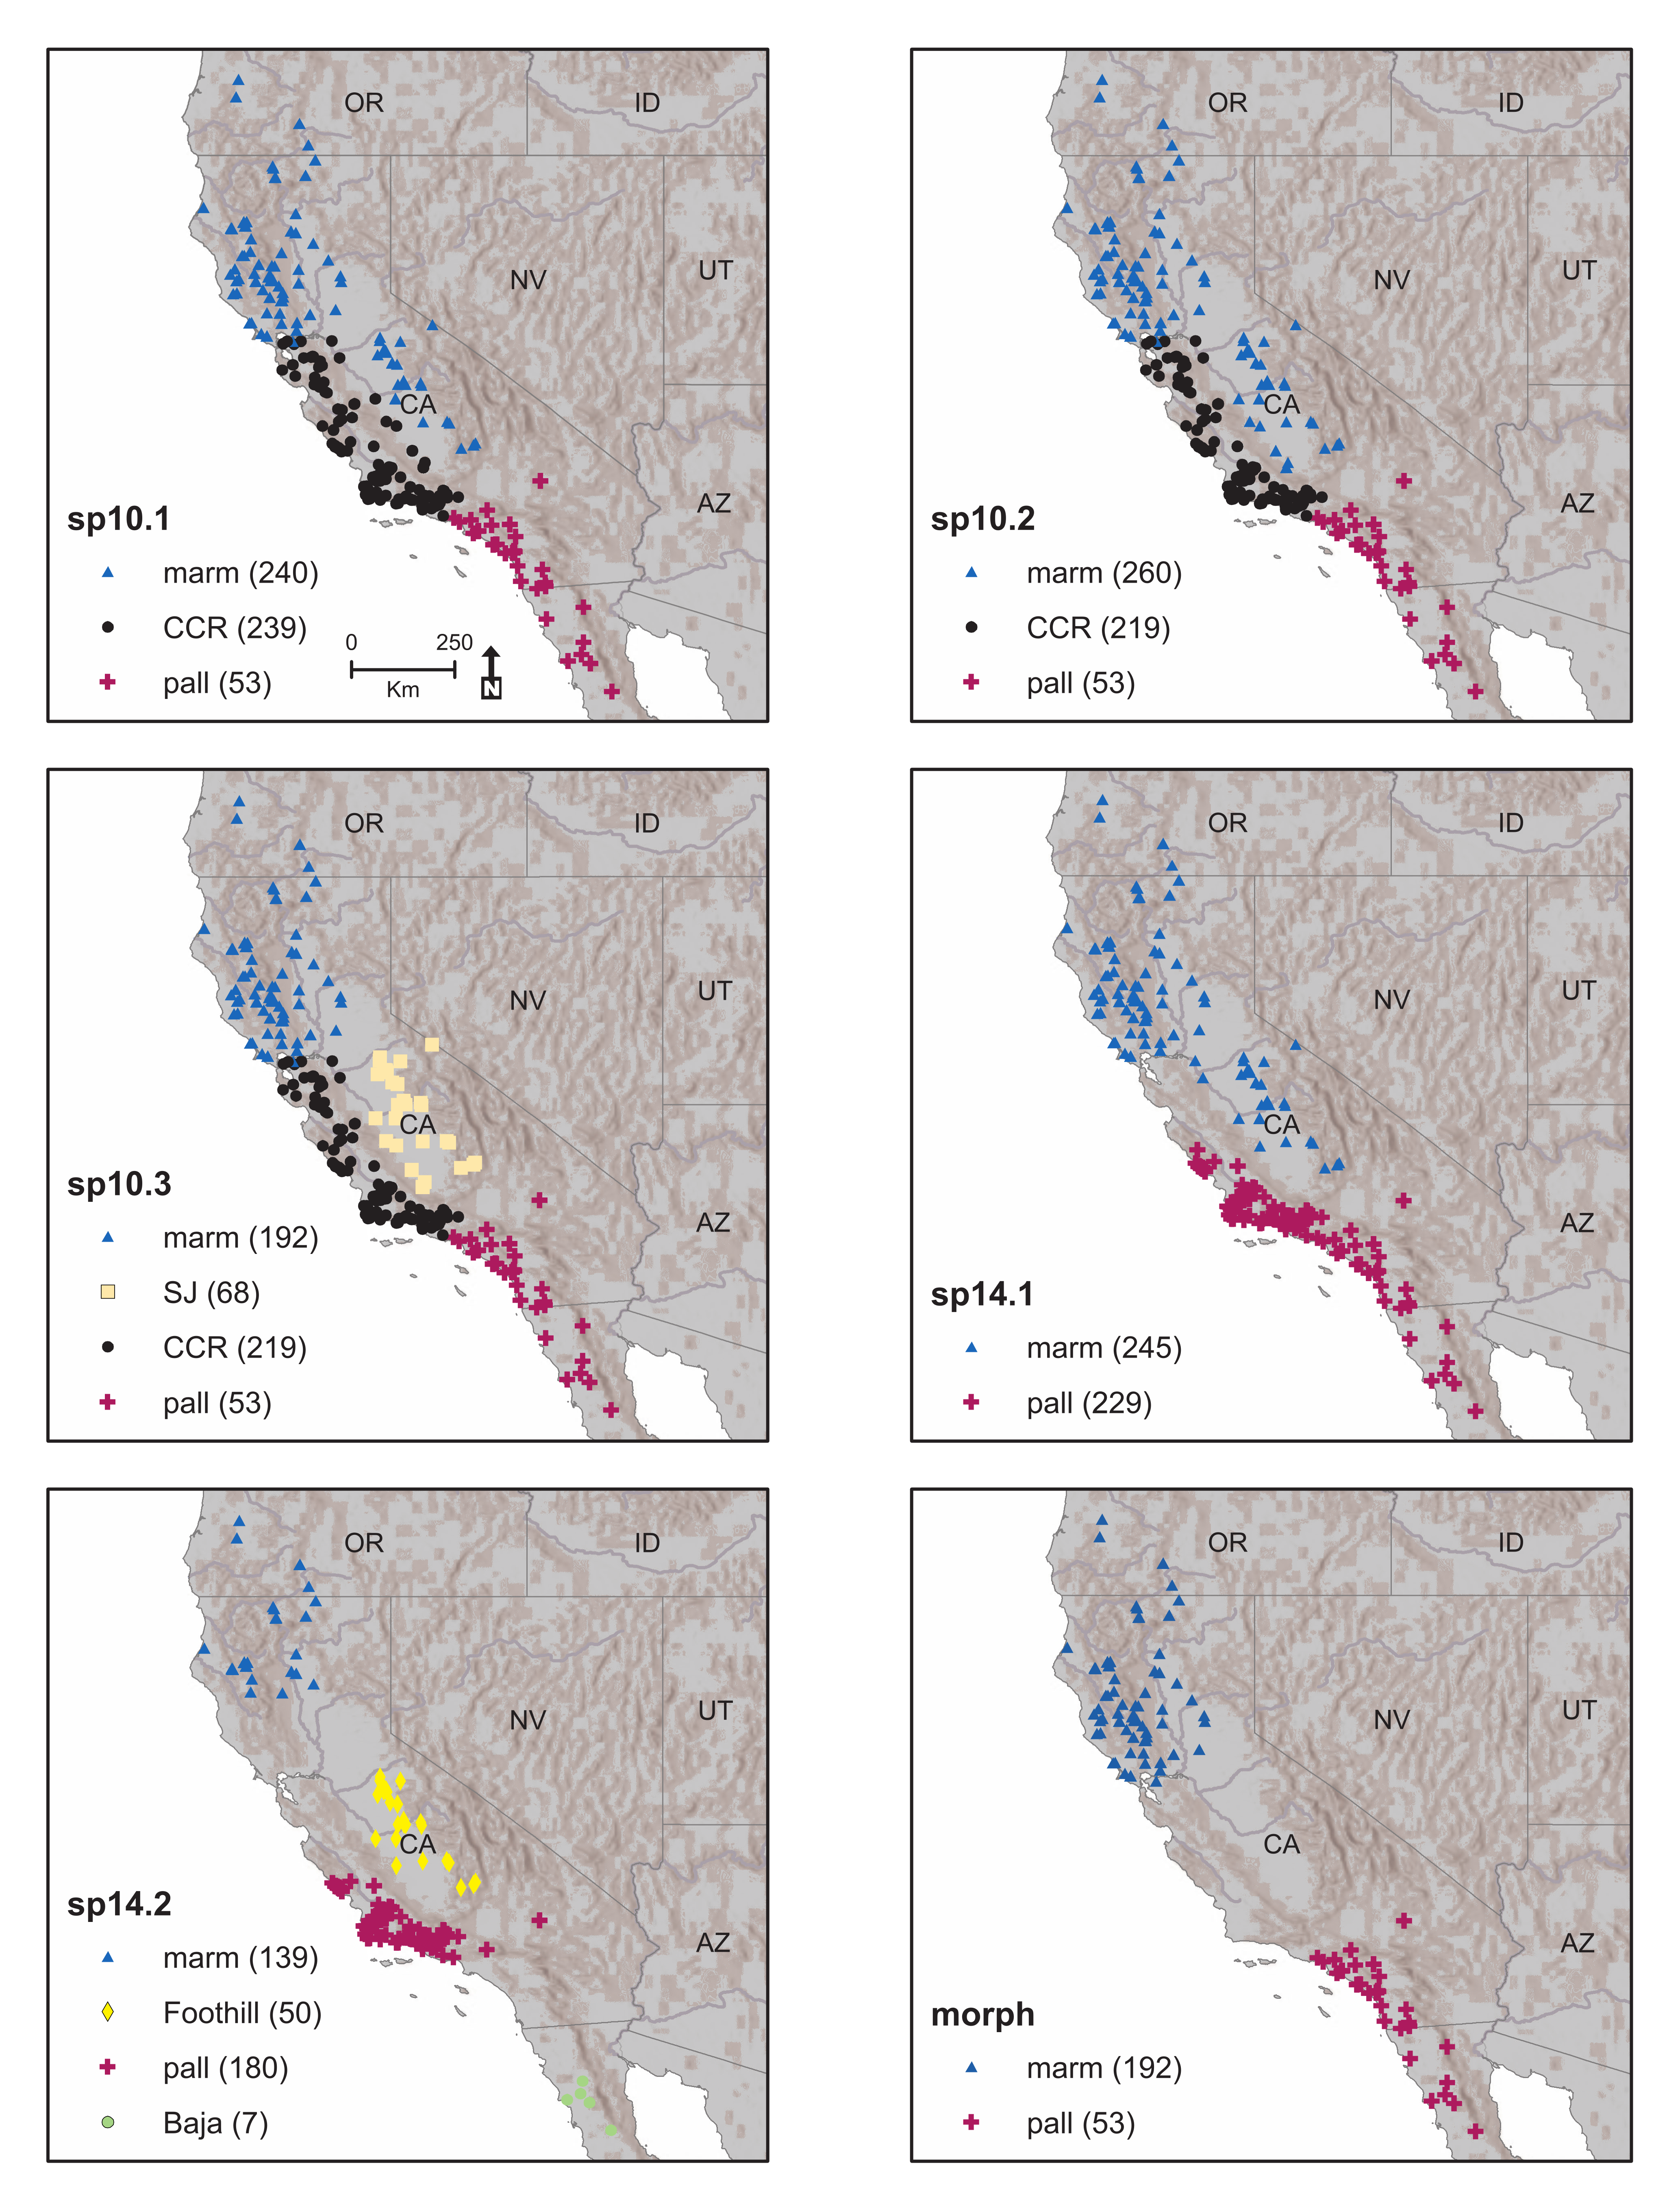
\includegraphics[height = 0.6\textheight, width = \textwidth, keepaspectratio = true]{figure/Ken_Ang_SpLoc_final_comp}
  \caption{Geographic distribution of specimens sampled for comparing the hypothesized subdivisions of \textit{Emys marmorata}. Each hypothesized scheme has two or more possible classes. Sample size differs between schemes because of our ability to confidently assign museum specimens to the various schemes. The number of localities shown on each map is less than the number of specimens sampled because some localities produced multiple specimens. The different classification abbreviations are as follows: \textit{E. marmorata} = ``marm'', \textit{E. pallida} = ``pall'', Central Coast Ranges = ``CCR'', San Joaquin Valley = ``SJ,'' Baya Peninsula = ``Baja,'', and Sierra Foothills = ``Foothill.''}
  \label{fig:map}
\end{figure}

\begin{figure}[h!]
  \centering
  \includegraphics[height = 0.6\textheight, width = \textwidth, keepaspectratio = true]{figure/plastra}
  \caption{Depiction of general plastral shape of \textit{E. marmorata} and position of the 19 landmarks used in this study. Anterior is towards the top of the figure.}
  \label{fig:plastra}
\end{figure}

\begin{figure}[h!]
  \centering
  \begin{subfigure}[b]{0.45\textwidth}
    \caption{}
    \includegraphics[height = 0.6\textheight, width = \textwidth, keepaspectratio = true]{figure/cc7_pc_graph}
  \end{subfigure}
  \begin{subfigure}[b]{0.45\textwidth}
    \caption{}
    \includegraphics[height = 0.6\textheight, width = \textwidth, keepaspectratio = true]{figure/tra_pc_graph}
  \end{subfigure}
  \caption{Two scatterplots of morphological differences from two of the three datasets analyzed in this study. (a) Scatterplot of the first two PCA axies from the landmarks from the eight different species dataset, and (b) the first two axes of variation from two subspecies of \textit{Trachemys} dataset. Point colors correspond to the categories within each dataset while point size is proportional to individual centroid size. In parentheses next to the axis labels are the percent of total variation accounted for by that axis. For both datasets there are clear distinctions between the different categories.}
  \label{fig:other_pca}
\end{figure}

\begin{figure}[h!]
  \centering
  \includegraphics[height = 0.6\textheight, width = \textwidth, keepaspectratio = true]{figure/emys_pc_graph}
  \caption{Scatterplot of the first two axes of morphological variation in the \textit{Emys marmorata} dataset. Each panel corresponds to one of the six different classification schemes analyzed as part of this study (Tab. \ref{tab:hypotheses}). Point color corresponds to the categories within each scheme, and the class names correspond to geographic regions. Point size is proportional to centroid size of that specimen and the numbers in parentheses next to the axis labels are the percent of total variation accounted for along that axis.}
  \label{fig:emys_pca}
\end{figure}

\begin{figure}[h!]
  \centering
  \includegraphics[height = 0.6\textheight, width = \textwidth, keepaspectratio = true]{figure/sex_test_hist}
  \caption{Comparison of observed Procrustes distance between the centroids of each sex (vertical line) to a null distribution generated from 1000 permutations of the sex-labels. This result indicates that the difference between the centroids is as small/smaller than expected by random.}
  \label{fig:sex_test}
\end{figure}

\begin{figure}[h!]
  \centering
  \includegraphics[height = 0.6\textheight, width = \textwidth, keepaspectratio = true]{figure/other_model_sel}
  \caption{Comparisons of model fit to the training dataset for each of the supervised learning methods applied to the first two datasets; the results from the eight species dataset are presented in the left column, while those from the \textit{Trachemys} dataset are presented in the right column. Models were fit to datasets of varying complexity, with the number of parameters listed along the x-axis. Model fit is measured as the area under the receiver operating characteristic (AUC), which ranges from 0.5 to 1. Error bars correspond to one standard error estimated from 10 rounds of 5-fold cross-validation. The red dot corresponds to the model fit with the highest mean AUC while the blue dot corresponds to the model selected for further analysis. In some cases, there is no difference in complexity between the best and selected models.}
  \label{fig:other_sel}
\end{figure}

\begin{figure}[h!]
  \centering
  \includegraphics[height = 0.6\textheight, width = \textwidth, keepaspectratio = true]{figure/other_oos_sel}
  \caption{The results of out-of-sample predictive performance of the selected models for both the eight species (left) and \textit{Trachemys} datasets. Predictive performance is measured as the area under the receiver operating characteristic (AUC), which ranges from 0.5 to 1. Points correspond to the individual out-of-sample predictive performance of the specific model, indicated along the x-axis. The horizontal bars correspond the average out-of-sample predictive performance of all the models.}
  \label{fig:other_oos}
\end{figure}

\begin{figure}[h!]
  \centering
  \includegraphics[height = 0.6\textheight, width = \textwidth, keepaspectratio = true]{figure/emys_model_sel}
  \caption{AUC values for models of varying complexity fit to the \textit{Emys marmorata} training datasets for each classification scheme. The x-axis corresponds to the total number of predictors included in each model, while the y-axis corresponds to the AUC value which is a measure of goodness of fit for classification datasets. A model with a high AUC value corresponds to better classification performance than a model with a lower AUC value. Standard errors on AUC estimates are calculated from 10 rounds of 5-fold cross-validation. Indicated are the best performing and the selected models, in red and blue respectively. In some cases, there is no difference in complexity between the best and selected models.}
  \label{fig:emys_sel}
\end{figure}

\begin{figure}[h!]
  \centering
  \includegraphics[height = 0.6\textheight, width = \textwidth, keepaspectratio = true]{figure/emys_oos_sel}
  \caption{Comparison of out-of-sample AUC estimates from the predictions of selected models (Fig. \ref{fig:emys_sel}), grouped by classification scheme. The horizontal line in each panel corresponds to the average AUC value across all models of that classification scheme.}
  \label{fig:emys_oos}
\end{figure}






%\subsection*{Online figure legends}
%
%\renewcommand{\thefigure}{A\arabic{figure}}
%\setcounter{figure}{0}
%
%\begin{figure}[h!]
%  %\includegraphics{jumps20m}
%  \caption{\textit{A}, the quick red fox proceeding to jump 20~m straight 
%  into the air over not one, but several lazy dogs. \textit{B}, the quick 
%  red fox landing gracefully despite the skepticism of naysayers.}
%  \label{Fig:Jumps}
%\end{figure}
%
%\begin{figure}[h!]
%  %\includegraphics{jumps-nr-okapi}
%  \caption{The quicker the red fox jumps, the likelier it is to land near 
%  an okapi. For further details, see \citet{LemKapEx07}.}
%  \label{Fig:JumpsOk}
%\end{figure}
%
%\renewcommand{\thefigure}{B\arabic{figure}}
%\setcounter{figure}{0}

\end{document}
